\documentclass[a4paper]{report}
\pagestyle{headings}
\usepackage{hyperref}
\usepackage{listings}
\usepackage{graphicx}
\usepackage{subfiles}
\usepackage{multirow}
\usepackage[table,xcdraw]{xcolor}
\lstset{numbers=right}
\lstset{breaklines}
\title{Lab Report for Software Engineering course \newline
 Lab 5: Demand Change and Prototype Development}
\author{Wang, Chen\qquad Liu, Jiaxing\qquad Huang, Jiani\qquad Tang, Xinyue \\
16307110064\qquad17302010049\qquad 17302010063\qquad 16307110476 \\
School of Software\\
Fudan University
}
\date{\today}
\bibliographystyle{plain}
\begin{document}
\maketitle

\tableofcontents
\chapter{Demands of this lab}
\section{Requirements of this lab}
According to the documentation of the lab assigner, this lab should satisfy the requirments in the following perspectives:
\subsection{Documentation}
In the documentation, we need to accomplish two parts, that is, we need to:
Understand the needs of this experiment, complete the requirements document;
Organize overall design documentation and detailed design documentation based on requirements.
\subsection{Code Style}
Before the experiment, our group members should agree on the code specification and the unified code style.
\subsection{Project Management}
The project is generally hosted on the Huawei Devcloud platform, on which platform we are going to finish the following tasks:
Project management should be arranged based on the DevCloud platform, including adding work items, assigning work items, associating work items, managing work item status, and other project management functions;
\par
Issues in the development process need to be recorded and managed on DevCloud, including defect reports in integrated development;
\par
Collaborative development based on Git, submit project documentation and code on a team basis.

\section{Background on the change of demand}
Starbubucks's coffee shop has received a large amount of financing and decided to open branches in different countries and regions.
\par
In order to adapt to the habits of users in different regions, it is necessary to develop a project prototype with basic functions, and then customize the system for different regions.Customized development needs to consider the following factors:
\subsection{Drink Customization}
At least 2 beverages need to be customized for local features (beverages defined in Lab4 are system default beverages).
\subsection{Currency change}
We need to switch to the corresponding currency according to different countries and regions, for example, a cappuccino in China 20CNY, a cappuccino in the US \$3 (do not consider currency exchange).
\subsection{Language change(localization)}
The system needs to switch the system language to the language of the corresponding country and region according to the language of different countries and regions. The range of language switching is visible to all system users (sales personnel) and customers (beverage buyers). For example, when the system user inputs, the input content should be the language of the corresponding country and region; after the order is successful, the customer sees The transaction content should be switched to the language of the corresponding country and region.
\subsection{Sales strategies}
A good sales strategy can bring huge benefits, and the system's default sales strategy is the sales strategy defined in Lab4. Because sales strategies can change as external markets change, systems are required to add and remove sales strategies in a pluggable manner.

\section{Specifications of the Lab}
The following requirements are to be met for the custom development factors described in the background in the previous section:
\subsection{Drink Customization}
Customize two beverages with reference to the previous lab implementation.
\subsection{Currency change}
There may be multiple currencies in different countries and regions. For example, Hong Kong can circulate Hong Kong dollars and Chinese Yuan, mainland China circulates Chinese Yuan, and the United States circulates US dollars. The prices of different currencies for the same item are different depending on the value of the product itself. The system needs to specify the corresponding price of the corresponding commodity for different currencies (the pricing of different currencies for each commodity, and the exchange rate pricing can be reasonably justified). Currently, the system only needs to support RMB and Hong Kong Dollar (HK\$).
\subsection{Language change(localization)}
Different countries and regions may have multiple official languages, and the system needs to switch between different languages according to different countries and regions. The system must be able to switch between English and Simplified Chinese.
\subsection{Sales strategies}
The sales strategy is added and deleted in a pluggable manner. The sales strategy in lab4 is the default sales strategy and cannot be deleted. The source of information for all sales strategies is order and system information (date and location). On the basis of lab4, the requirements of (1)(2)(3) and the pluggable components of the sales strategy can be regarded as the prototype of the project.Based on this prototype, add the following sales strategy:
\begin{enumerate}
\item
When the time zone of the system is November 11th, the total price of all commodities (including all prices) will be 50\% off.
\item
When the order contains at least one tea item and at least one item of the Coffee category, the total price (including all prices) is 15\% off.
\end{enumerate}

\section{Additional precautions of this lab}
\subsection{Switch interface of currency and language}
The switching of currency and language can depend on a ``switch'', which is an abstraction rather than a concrete implementation, since the opening and closing of the switch may depend on different external conditions.
\subsection{Prototype-based development}
The addition and deletion of the sales strategy is based on the fact that the prototype of the project has been developed, and the sales strategy is added and deleted through the interface of the sales strategy provided by the prototype. When using the prototype, you can't modify the code of any prototype, and you can only perform secondary development on the basis of the prototype.
\subsection{Methods for switch and pluggable components}
The development of "switches" and pluggable components can refer to the relevant materials.
\subsection{Freedom of change of the existing frameworks}
In order to flexibly realize the four requirements in the previous sections above, it is encouraged that every team should design independently. The fields and method signatures in the framework code provided by the assistants in Lab4 can be modified. It should be emphasized that after the prototype is completed, it cannot be modified, and it can only be developed on the basis of the prototype.
\chapter{Division of work for this lab}
\section{Division of work: Wang, Chen}
\subsubsection{(Git username: \emph{Wang, Chen}; Student ID: \emph{16307110064})}
He constructs the overall structure of the project, divides the entire workload into several parts so that each part can be finish the work separately. In addition, he draws the diagram of the entire project on the Huawei cloud platform that contains the parts like Epic, feature, story and tasks. Furthermore, he scratches the outline of how to implement the methods adopted in this project. At last, he summarized the general parts in the documentation and drafted some regulations for commit messages.

\section{Division: Huang, Jiani}
\subsubsection{(Git username: \emph{Currycurrycurry} Student ID: \emph{17302010063})}
She implements the concrete methods in the language and currency switch feature.

\section{Division: Tang, Xinyue}
\subsubsection{(Git username: \emph{xinyuetang} Student ID: \emph{16307110476})}
She implements the methods related to order processing, discount processing and total price processing.

\section{Division: Liu, Jiaxing}
\subsubsection{(Git username: \emph{jiaxingliu} Student ID: \emph{17302010049})}
He designed the interfaces for various modules of the project including the \emph{menu} module and the \emph{language} module. In addition, considering the actual circumstances of the product, he adopts the \textbf{singleton} design pattern, the \textbf{strategy} pattern so as to improve the encapsulation level and the ability for extension of the application. 
\par
He also finishes the testing work of the entire project, whose work  is an important foundation of the \emph{Test-Driven Development} of the project. In particular, he realizes the \emph{JUnit} test cases within the project and the \emph{Swagger} interface test of the project on the Huawei Cloud Platform.

\chapter{Analysis of the demands}
\section{General analysis of the demands}
In this version of requirement, a series of new functions are proposed and they are supposed to bring the general construction of the project some prominent change. Specifically, the requirements of the project lie in two perspectives: a prototype that should work for the all future new regions and two detailed and concrete implementations for the region of China and Hong Kong specifically.
\par
Therefore, the main work of this project has two stages:
\begin{enumerate}
\item
Design and determine our project prototype;
\item
Continue finishing the specified work and implementing the corresponding functions based on the prototype.
\end{enumerate}
\par
Therefore, in the following paragraphs, I will try to analyze the demands from the two stages shown above.

\section{General workflow}
According to the general analysis in the previous section, the total workflow of this project can be shown as the following diagram.
\begin{figure}
  \centering
  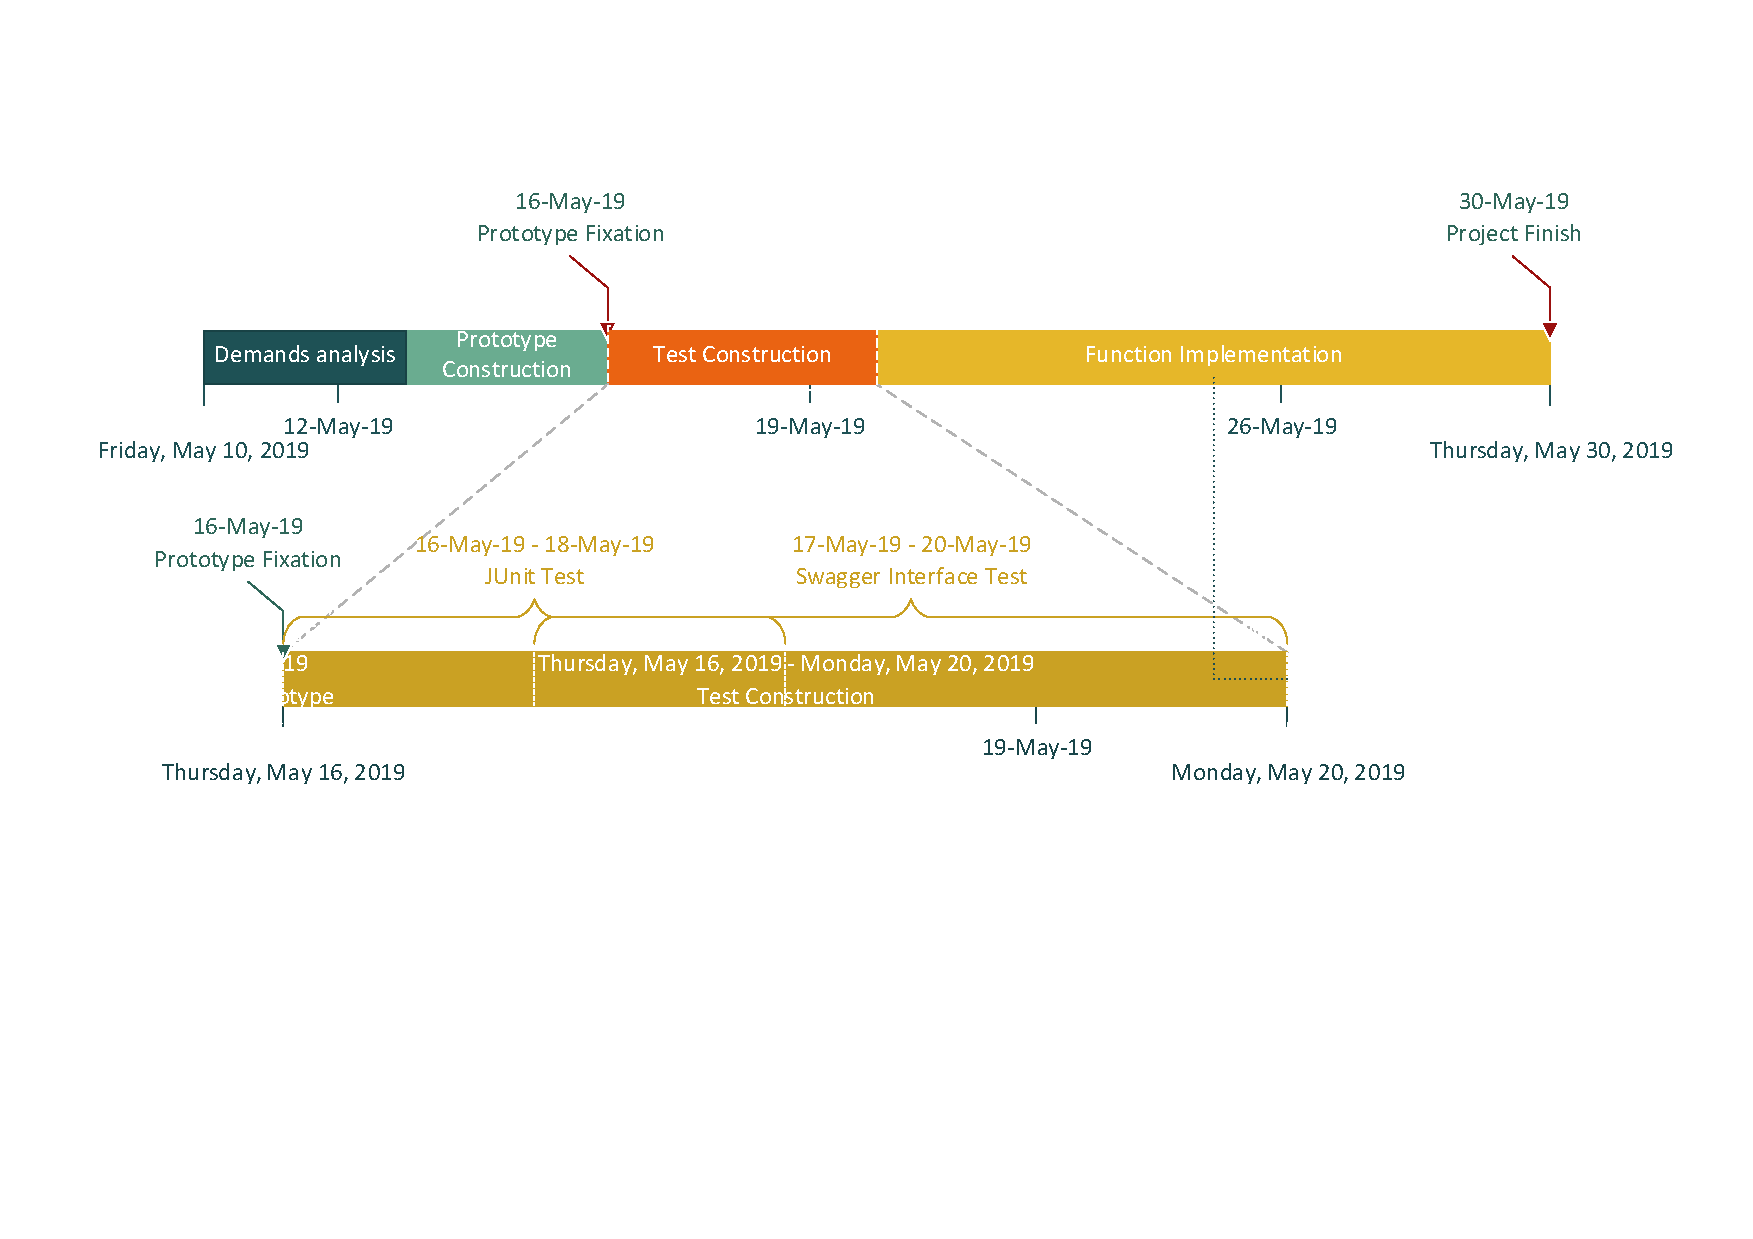
\includegraphics[scale=0.45]{workFlow.pdf}
  \caption{Overall workflow}\label{1}
\end{figure}

\section{Project Prototype}
In the requirement documentation, it is clearly specified that our project should have a clear prototype and continue with the future works based on the existing prototypes. Therefore, the first step for the team members to do is to finish the prototype. 
\par
The prototype need to well represent the newly-added features that will be future implemented. Specifically, the prototype should have all the necessary interfaces needed for the customized drink, the currency switch, the language switch and the strategy change.
\par
Should there be future concrete implementation on the futures above, the developers (our team members here) should only need to add new classes implementing the interfaces without modifying the existing interfaces.
\section{Currency switch analysis}
The requirements of currency switch has a lot to be further analyzed before concrete implementation. As the features of the project display, each drink and its corresponding ingredients have a price. The prices will be used in the order information and later be used to charge from the customers. However, different region has different currencies, while the drink item will also vary from one region to another. Therefore, the price of the order items should not be written directly into the code any more, which can lead more complexity to future feature extension. 
\par
Considering we are running a Spring Application, which allows a wide range of property resources lying in the \emph{resources} folder of the application with a file extension \emph{properties}, the price information of the order items are suitable to be stored in such places. 
\par
In such way, the price information of the project is depleted from the code section and it is much easier to maintain the data. Furthermore, should new currencies be supported in the future, we also have no need of input the price information in the code, and only need to append the configuration files.
\section{Language switch}
The switch of language is a common requirement in all the international software. To improve maintainability and readability, in addition to reduce future cost of maintenance, all the display language tags are stored in some files as constants. For example, in Android applications, all the \emph{String}s that need to be displayed are encouraged to be saved into a separate XML file and then read via the constant names. Meanwhile, the the global language switch, either controlled by the Android Operating System or controlled by the application, can determine which \emph{String} to be displayed. That is, the same display info are stored and accessed via the same variable name, while the variables direct the application to different files when different languages are set. 
\par
Therefore, in our application, we are encouraged to store the display information via constants and a global language switch can determine which language's constant will be transferred to the application.
\section{Sales strategies}
Sales strategy is an important part of the application. However, in order to better utilize the market, sales strategies need to be easily switched on or off from the pricing services.
\par
Considering such circumstances, each sales strategy need to be a single extract-able method or class so that in the future configuration, we can add on or off such strategies with ease.


\chapter{General design for the implementation}



\chapter{Detailed design for the implementation}
\section{Test design: for Test-Driven Development}
\subsection{Test components of the project}
In this project, we have various types of tests so as to ensure that all components are working properly.
\par
Specifically, we have JUnit test to be utilized during the initial stages of development. These unit tests give clear guidance of the project.
In addition, we have utilized the Huawei Cloud platform with its strong Interface test function. The interface test function enables the entire project can function well with its public interfaces. What's more, the interface tests are integrated into the project as Swagger Interface test component. In this component, there is a standalone package that has a front-end user interface and will be convenient to present interface test locally.
\subsection{Swagger Interface Test}
The front-end user interface of the local Swagger Interface Test is shown as the following figures(Figure \ref{2} and Figure \ref{3}):

\begin{figure}
  \centering
  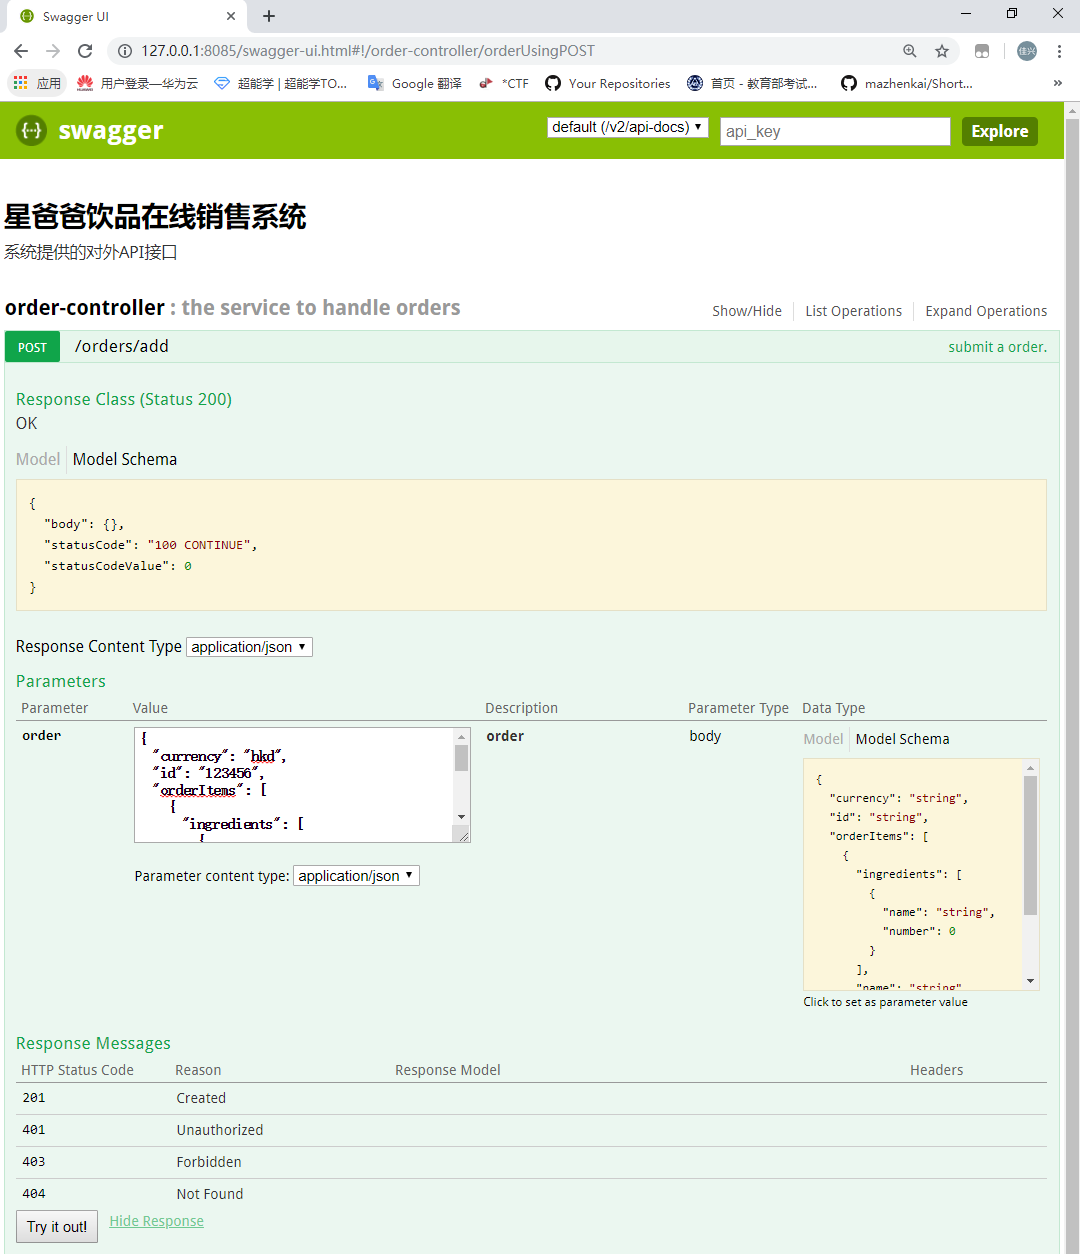
\includegraphics[scale=0.45]{swagger2.png}
  \caption{Overall workflow}\label{2}
\end{figure}

\begin{figure}
  \centering
  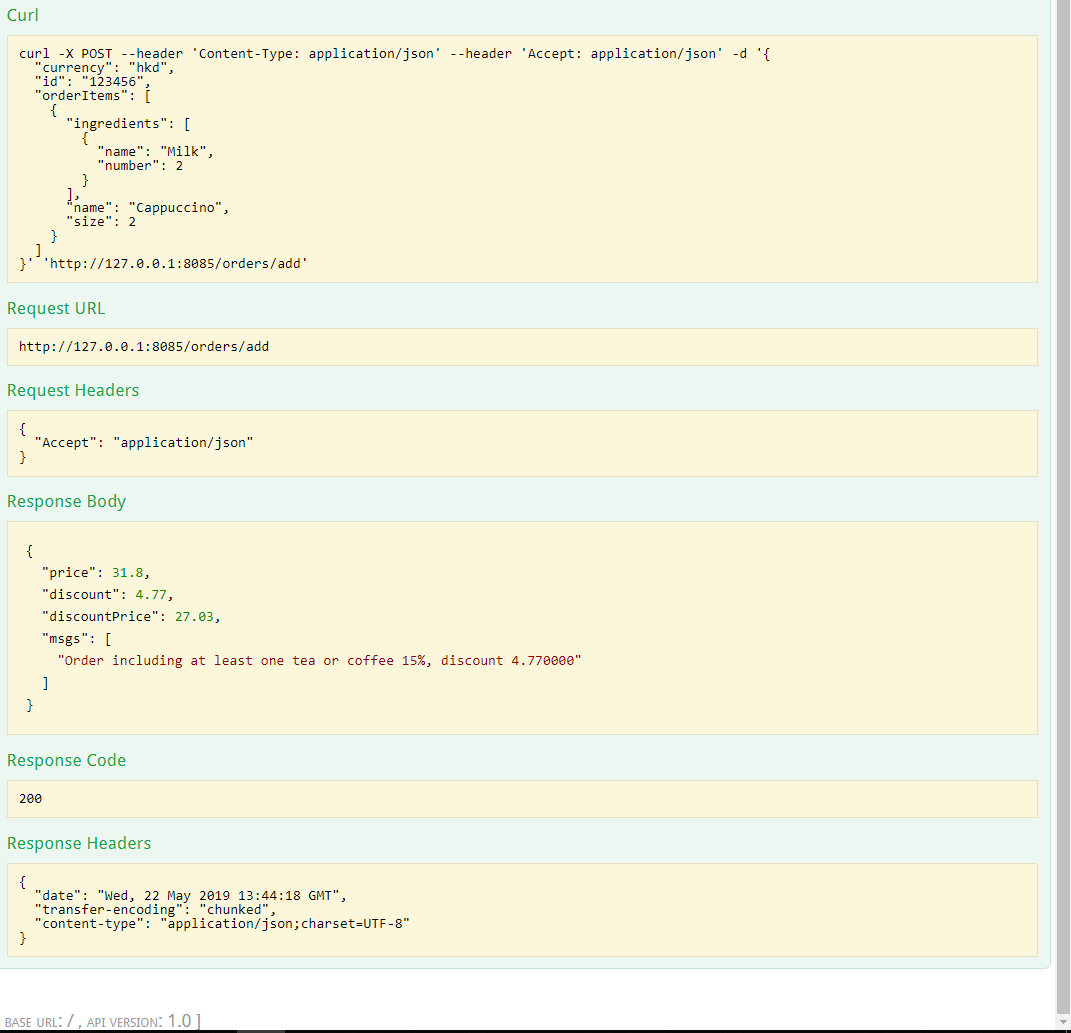
\includegraphics[scale=0.45]{swagger1.png}
  \caption{Overall workflow}\label{3}
\end{figure}

%Huang Jiani 2019-5-20 below%
\section{Switch Language Implementation}
\par The switch of language will be mainly displayed in the user interface, so all the information that need to be multi-translated will be separately placed into  different constant files. In this iteration of implementation, we only instantiate the Chinese and English versions. And the correspondent service classes will use a typical mechanism called reflection to implement the switch of different constant language files.
\par In the following two sections, the detailed design of constant files and language service classes will be respectively clarified.
\subsection{Language Constant Files}
\par The two constant files are positioned in the constant package. In these two files, all the variables (there are no methods) are qualified with public static final String since they are all constant strings.
\par To our attention, all the necessary variables should have the same names in all the language files to maintain the availability of reflection.
\subsection{Language Service Classes }
\par To follow the idea of prototype development, all the concrete service classes should implement their corresponding interfaces. The interface make it clear what the service will implement and its parameters. The most notable design pattern in this class is single-instance pattern.

\section{Switch Currency Implementation}
\subsection{Currency Property Files}
\subsection{Currency Service Classes}
%Huang Jiani 2019-5-20 above%


\chapter{Problems encountered in this project}
\section{Problems in coding}
\subsection{Wrong usage of built-in menu item price}
\par When testing the strategy of \emph{CombinationDiscountStrategy}, it occurs an error. The discount is illegal when the currency is hkd. Therefore, I create a work item \#2282258. After checking the implementation of the class, I found the reason. In fact, there may be more than one error, but of the same type. For example, according to the strategy, when there are two cappuccino, we can get the second one for half price. But the involved method just returns a discount of 11 yuan and it is illegal. When the currency is hkd, the discount is 12.5 hkd. So in order to cope with the problem, we use the method \emph{menuService.getPrice(Ljava/lang/String,Ljava/lang/String):LD} to replace the built-in price. And the error disappered.
\subsection{Wrong usage of \% in a format string}
\par According to the strategy of \emph{TeaAndCoffee15OffStrategy}, when the order consists of one for coffee or tea, we can get drinks \%15 off. So in the payment information, there may be a character of \%. In most time, it is ok. But a \% in the format string may be illegal, especially in the format string formatting by \%d, \%f or something else. In this format string, we should use \%\% to replace \%. In fact, it is just an easy question, but not least.
\subsection{Problems in applying swagger testing}
\par In the project, we use two tests, one for \emph{Junit} and one for \emph{Swagger}. \emph{Junit} testing is much easier than the second one, we just need to add some test classes. Before using \emph{Swagger} testing, we use an interface testing for a special url in the cloud of huawei. But the interface testing is inefficient and there is a bad management for it, so we deside to use \emph{Swagger} testing. But it is not essay, First, I need to know what is \emph{Swagger} testing and how to use it. After learning it, I found it is a set of interface testing case and it can be imported to a script, so it is essay to manage. But when I attempted to use it, some problems occur. First, I should add the dependency of the \emph{Swagger} to the file \emph{pom.xml}, which would load some classes when the program works. And then, to use it, I should make some annotations. And the following are some examples.
\begin{lstlisting}[language=java]
@RestController
@RequestMapping("/orders")
@Api(value="order",description = "the service to handle orders")
public class OrderController {

    @Autowired
    private OrderServiceImpl orderServiceImpl;

    @RequestMapping(value="/add",method= RequestMethod.POST,produces = "application/json")
    @ApiOperation(value = "submit a order.",response = ResponseEntity.class)
    public ResponseEntity<PaymentInfo> order(@RequestBody @Valid Order order) {
        ArrayList<MarketingStrategy> strategies = new ArrayList<>();
        strategies.add(new DoubleElevenStrategy());
        strategies.add(new CombinationDiscountStrategy());
        strategies.add(new FullDiscountStrategy());
        strategies.add(new TeaAndCoffee15OffStrategy());
        orderServiceImpl.setStrategies(strategies);
        return ok().body(orderServiceImpl.pay(order));
    }
}
\end{lstlisting}
\begin{lstlisting}[language=java]
@ApiModelProperty(notes="order ID",required = true,dataType = "String")
private String id;

@ApiModelProperty(notes="order items",required = true,dataType = "OrderItem")
private List<OrderItem> orderItems;

@ApiModelProperty(notes = "the currency",required = true,dataType = "String")
private String currency;
\end{lstlisting}
\par In the second example, I worked out an important problem. In the second annotation, I am confused about what the dataType should be because the dataType of \emph{ApiModelProperty} only consists of some basic types, such as int, string, double and stuff. After searching for the solution for minutes, I still didn't find the right answer. And I deside to assign \emph{OrderItem} to it and make annotations for the class \emph{OrderItem}. Luckily, it works well. So I finished using \emph{Swagger} testing.
\section{Problems in designing the project's structure}
\subsection{Problem in applying xml files}
\par Being influenced by the arrangement of constants in \emph{android} projects, I often want to use \emph{xml} files to cache some constants. But after I tried some methods to do so, I found it is much more complex than using \emph{properties} files, which is well supported by \emph{java virtual machine}. So to be easy, we use \emph{properties} files to cache menu and some important constants.
\subsection{Wrong design of interface in \emph{MarketingStrategy}}
\par In the interface \emph{MarketingStrategy}, there is an important method called \emph{getDiscount(Lfudan/se/lab4/dto/Order):Lfudan/se/lab4/dto/PaymentInfo}. Now the method is well designed. But at first, I design the return value to be a double value. And if so, to get the payment information, the program may do ssame thing in another position and it is inefficient.
\chapter{Measures against demand change}



\chapter{Tools and literature involved in this project}



\chapter{Conclusion for the process of accomplishing this project}


\begin{thebibliography}{A}


\bibitem{1}
Wikipedia contributors. (2019, March 22). JUnit. In \emph{Wikipedia, The Free Encyclopedia}. Retrieved 14:53, April 1, 2019, from \url{https://en.wikipedia.org/w/index.php?title=JUnit&oldid=888928403}

\end{thebibliography}
\end{document} 